\section{Works Completed}
\begin{frame}{System Setup and Environment Configuration}
\begin{itemize}
    \item Linux-based development environment (Arch Linux)
    \item Mininet 2.3.1b4 for network emulation
    \item Ryu controller with Python 3.9 (via pyenv)
    \item Open vSwitch with OpenFlow 1.3 enforced
    \item Controller–switch communication verified on port 6653
\end{itemize}
\end{frame}
\begin{frame}{Environment Verification}
\begin{figure}
    \centering
    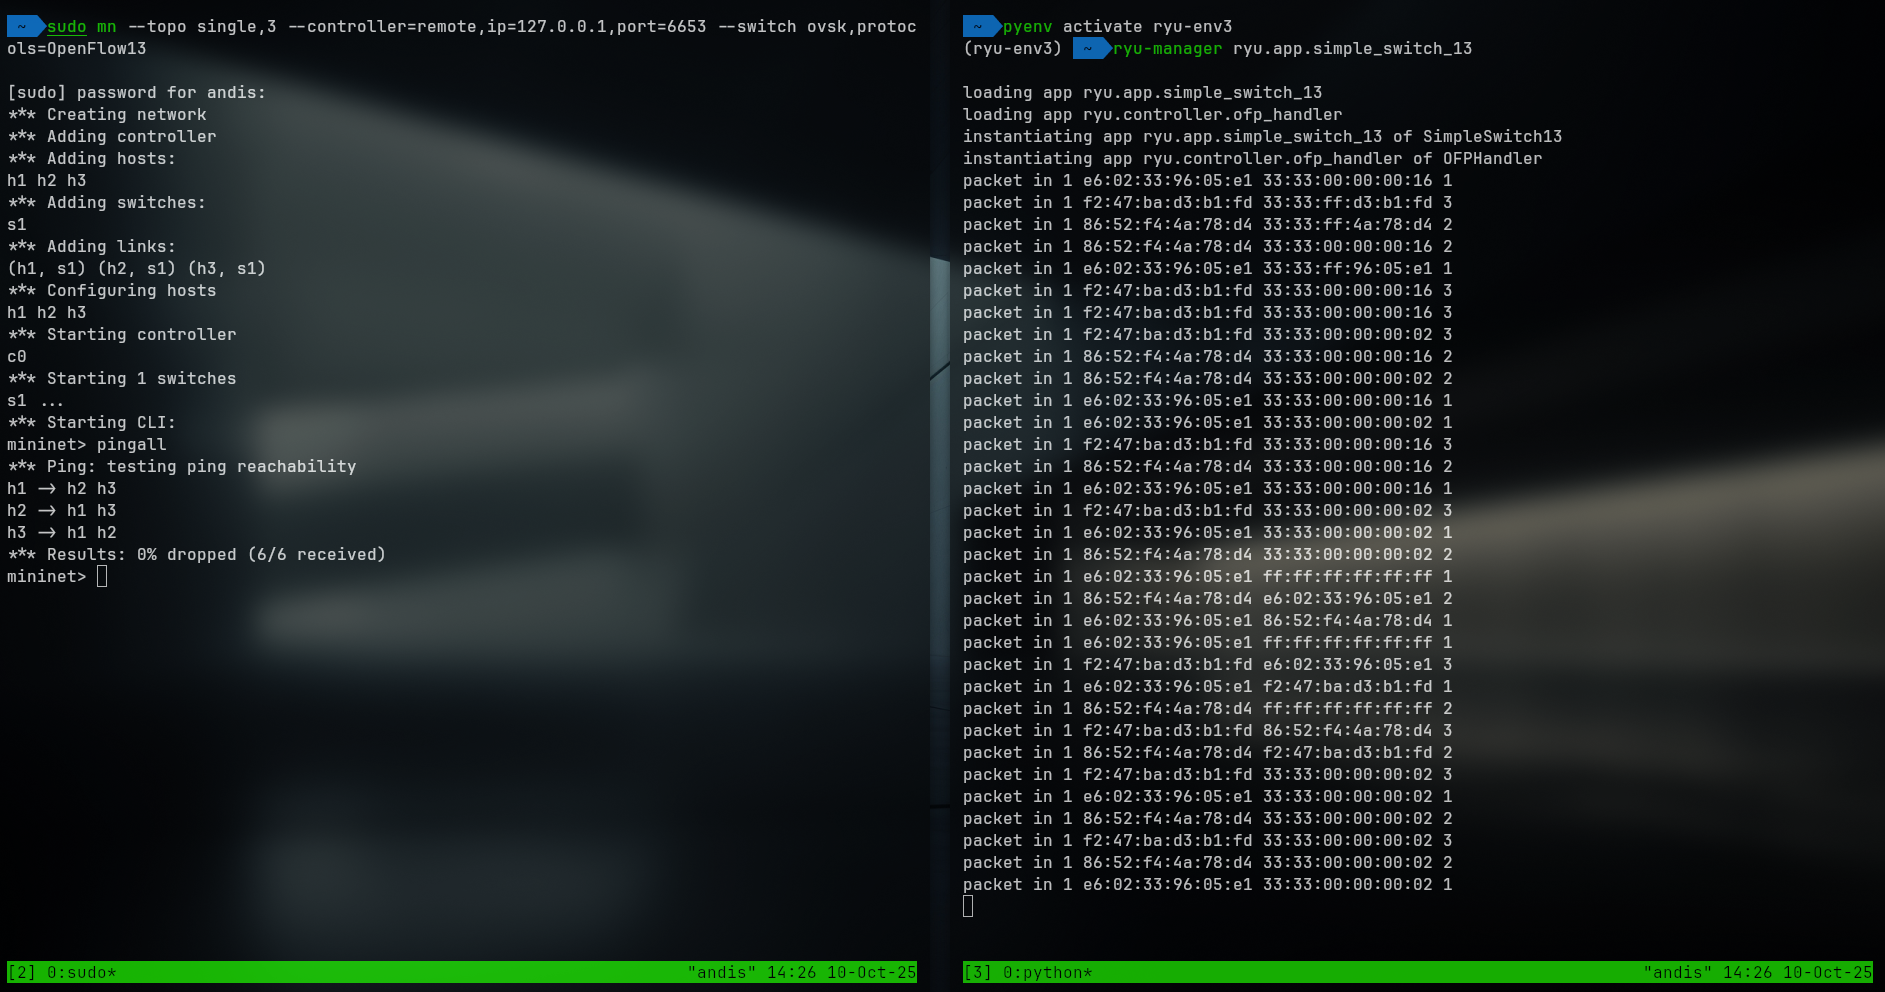
\includegraphics[width=0.7\linewidth]{Images/setup_environment.png}
    \caption{Mininet and Ryu Controller Running Successfully}
\end{figure}
\end{frame}
\begin{frame}{Topology Design and Implementation}
\begin{itemize}
    \item Custom Python script for Fat-Tree topology
    \item Parameter: $k = 4$
    \item Simulates data-center scale network
    \item Hierarchical design: Core, Aggregation, Edge
\end{itemize}
\end{frame}
\begin{frame}{Fat-Tree Topology Structure ($k=4$)}
\begin{itemize}
    \item Core switches: 4
    \item Aggregation switches: 8
    \item Edge switches: 8
    \item Hosts: 16
    \item Designed for high path diversity and scalability
\end{itemize}
\end{frame}
\begin{frame}{Fat-Tree Topology Visualization}
\begin{figure}
    \centering
    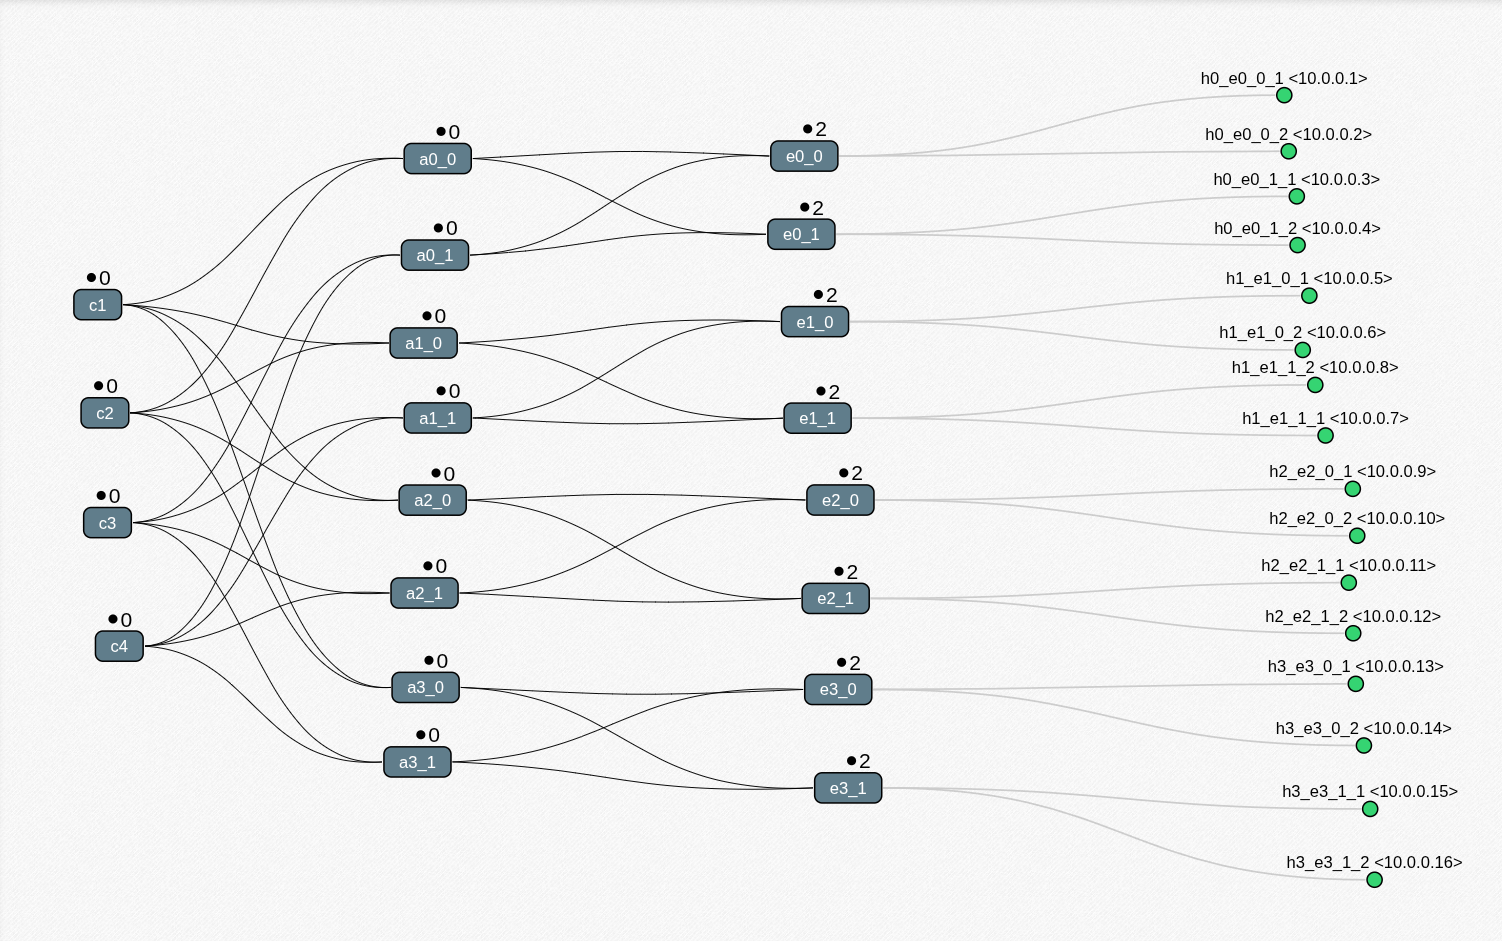
\includegraphics[width=0.7\linewidth]{Images/fat_tree_topology.png}
    \caption{Mininet Fat-Tree Topology ($k=4$)}
\end{figure}
\end{frame}
\begin{frame}{Controller Development}
\begin{itemize}
    \item \textbf{SimpleSwitch13}
    \begin{itemize}
        \item OpenFlow 1.3 learning switch
        \item MAC learning and packet-in handling
    \end{itemize}
    \item \textbf{Enhanced Learning Switch}
    \begin{itemize}
        \item Idle and hard timeouts
        \item LLDP filtering
        \item Precise flow matching
    \end{itemize}
\end{itemize}
\end{frame}
\begin{frame}{Controller Testing and Validation}
\begin{figure}
    \centering
    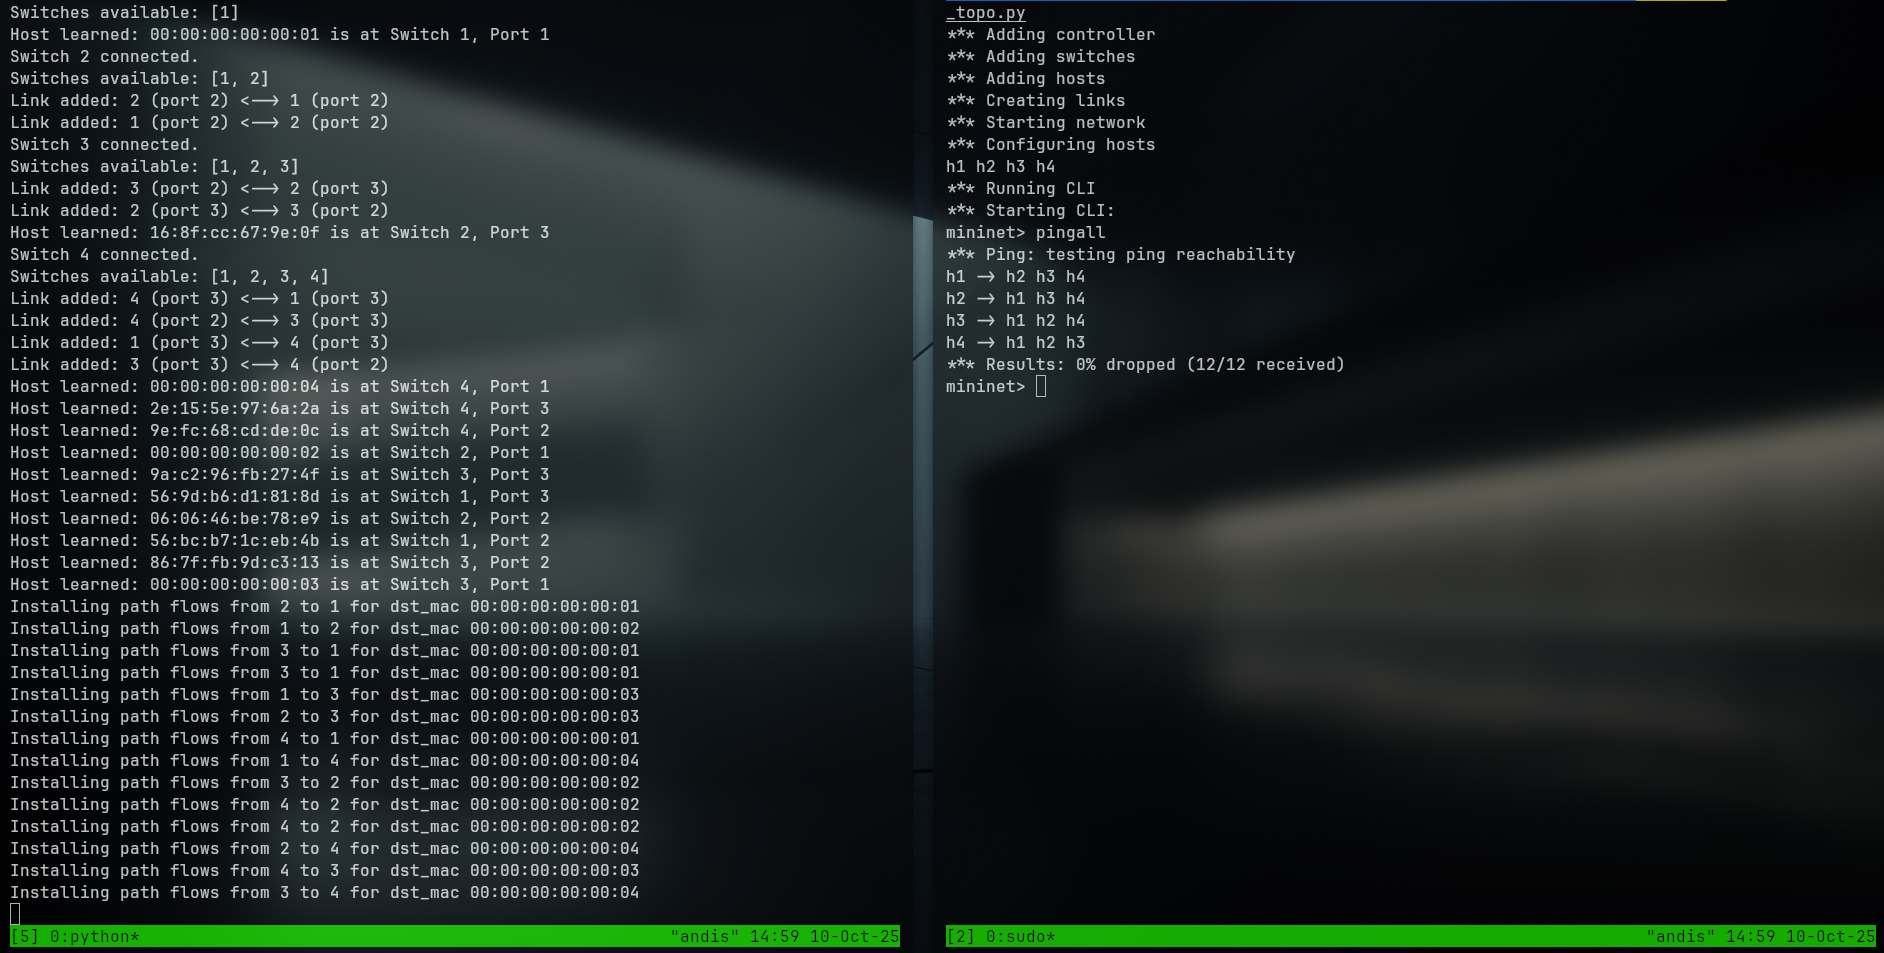
\includegraphics[width=0.7\linewidth]{Images/controller_ping.png}
    \caption{Successful Ping Test in Small SDN Topology}
\end{figure}
\end{frame}
\begin{frame}{Network Monitoring Implementation}
\begin{itemize}
    \item Developed \texttt{NetworkMonitor} Ryu application
    \item Periodic polling of:
    \begin{itemize}
        \item Port statistics
        \item Flow statistics
        \item Packet and byte counters
    \end{itemize}
    \item Enables congestion and utilization analysis
\end{itemize}
\end{frame}
\begin{frame}{Real-Time Monitoring Output}
\begin{figure}
    \centering
    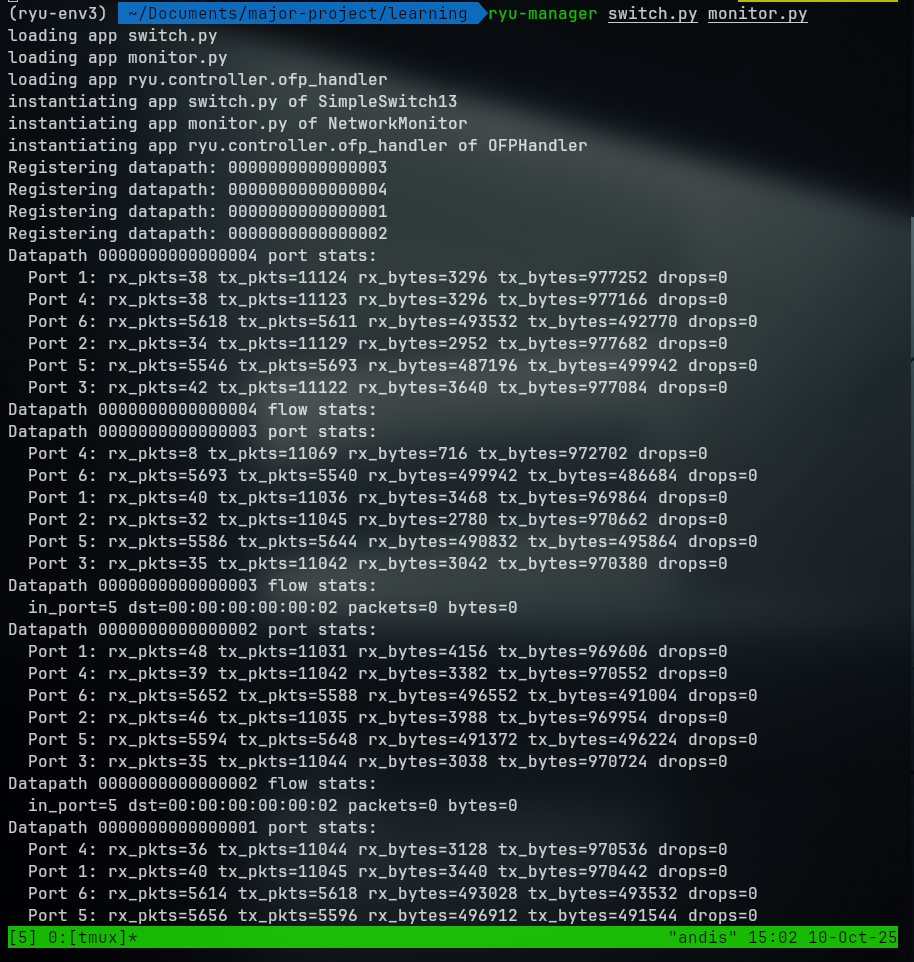
\includegraphics[width=0.7\linewidth]{Images/network_monitor.png}
    \caption{Live Port and Flow Statistics Collection}
\end{figure}
\end{frame}
\begin{frame}{Traffic Generation Setup}
\begin{itemize}
    \item ApacheBench used for realistic client behavior
    \item Traffic patterns:
    \begin{itemize}
        \item Constant
        \item Bursty
        \item Incremental
    \end{itemize}
    \item Enables stress-testing of load balancer
\end{itemize}
\end{frame}
\begin{frame}{Traffic Patterns}
\begin{figure}
    \centering
    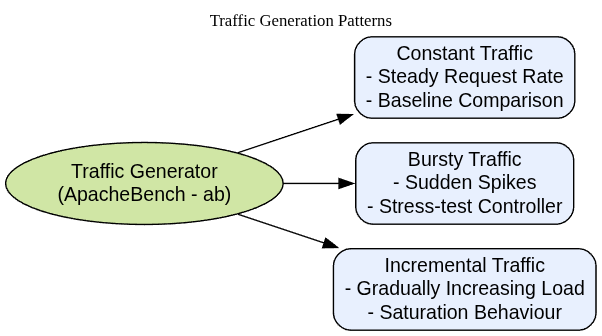
\includegraphics[width=0.7\linewidth]{Images/traffic_patterns_placeholder.png}
    \caption{Traffic Load Patterns Used for Training}
\end{figure}
\end{frame}
\begin{frame}{Controller Initialization}
\begin{itemize}
    \item Virtual IP successfully registered
    \item Backend server pool initialized (h1, h2, h3)
\end{itemize}

\begin{figure}
    \centering
    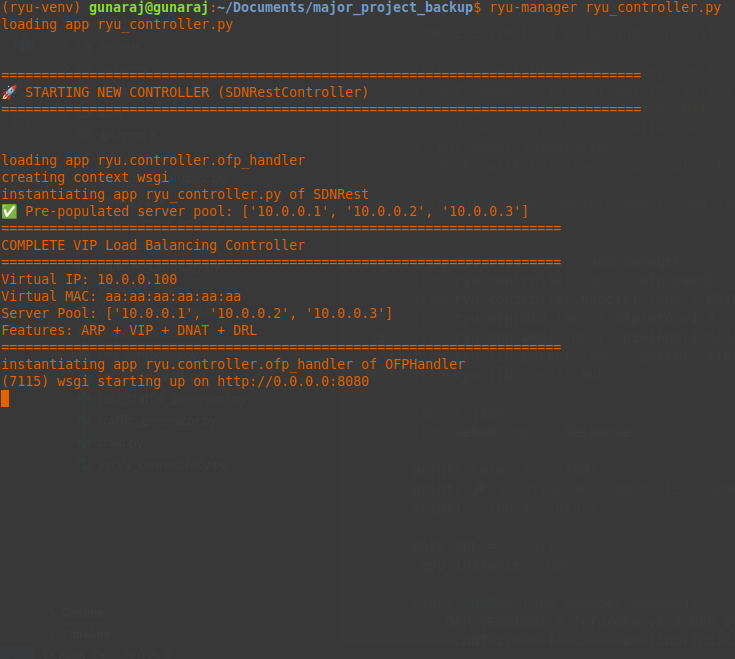
\includegraphics[width=0.6\linewidth]{Images/init.png}
    \caption{Controller Initialization Logs}
\end{figure}
\end{frame}
\begin{frame}{Routing Installation}
\begin{itemize}
    \item Static routing used for baseline connectivity
    \item 921 flow rules installed
    \item Ensures full reachability before DRL decisions
\end{itemize}

\begin{figure}
    \centering
    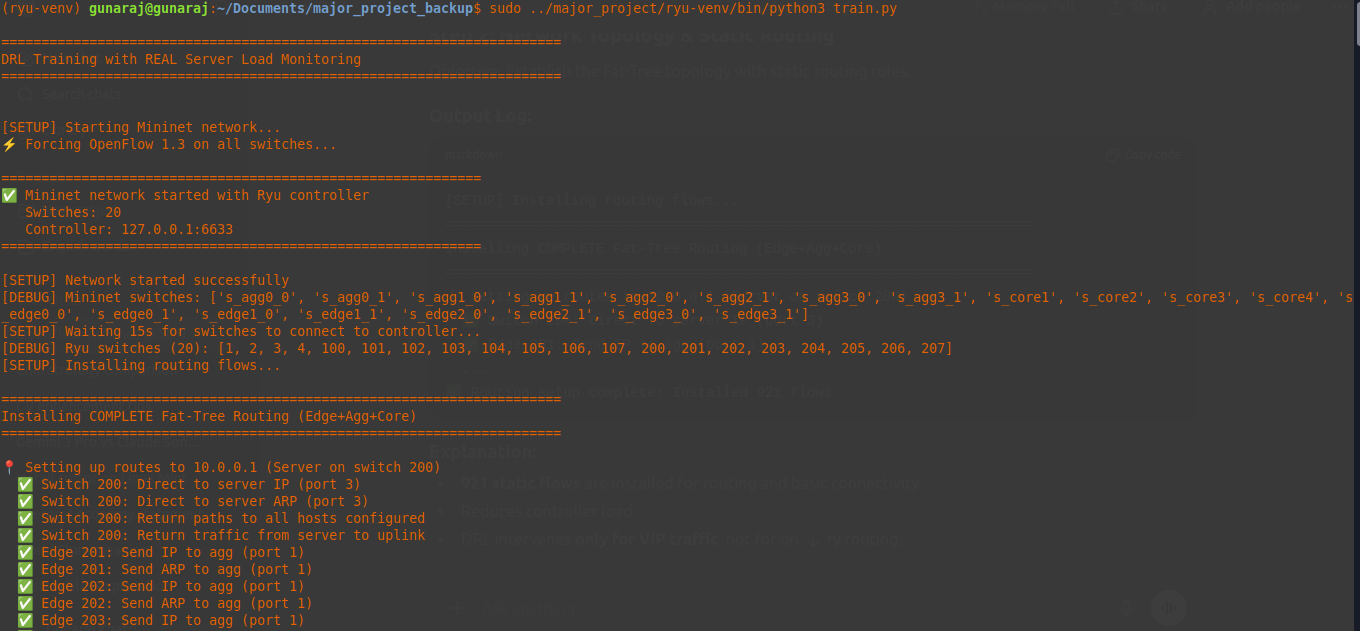
\includegraphics[width=0.6\linewidth]{Images/route_init.png}
    \caption{Static Routing Initialization}
\end{figure}
\end{frame}
\begin{frame}{Real-Time DRL Decision Making}
\begin{itemize}
    \item DRL agent selects server per request
    \item Decisions based on real-time metrics
    \item Integrated with Ryu via REST APIs
\end{itemize}

\begin{figure}
    \centering
    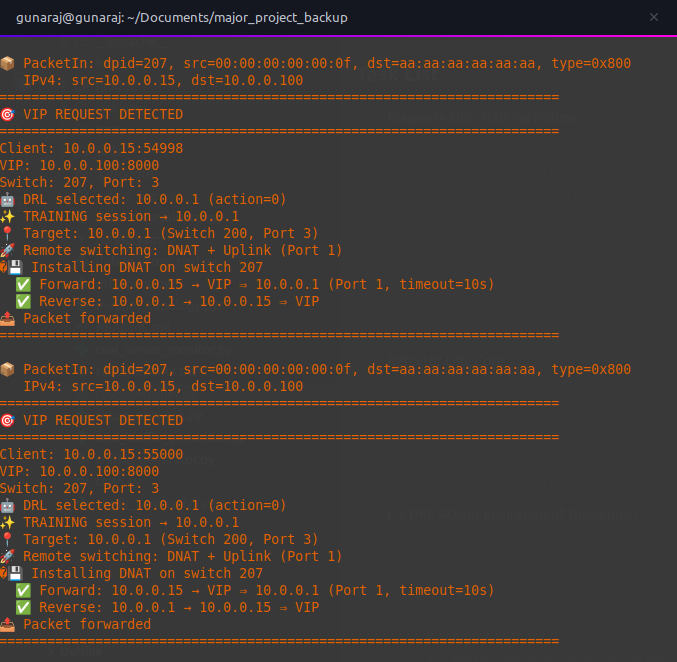
\includegraphics[width=0.5\linewidth]{Images/drl.png}
    \caption{DRL Agent Decision Logs}
\end{figure}
\end{frame}


% ================= Q LEARNING =================
\begin{frame}{Neural Network Implementation}

\begin{figure}
    \centering
    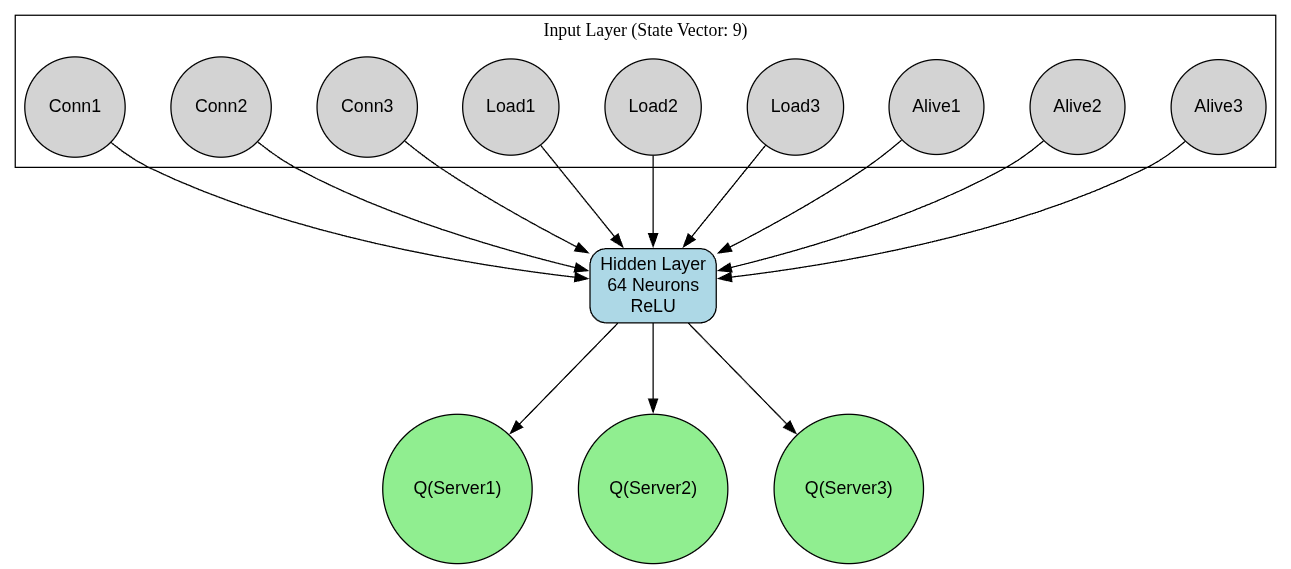
\includegraphics[width=0.75\linewidth]{Images/neuralnet.png}
    \caption{Neural Network}
\end{figure}
\end{frame}

% ================= SYSTEM INTEGRATION =================

\begin{frame}{System Integration}
\begin{figure}
    \centering
    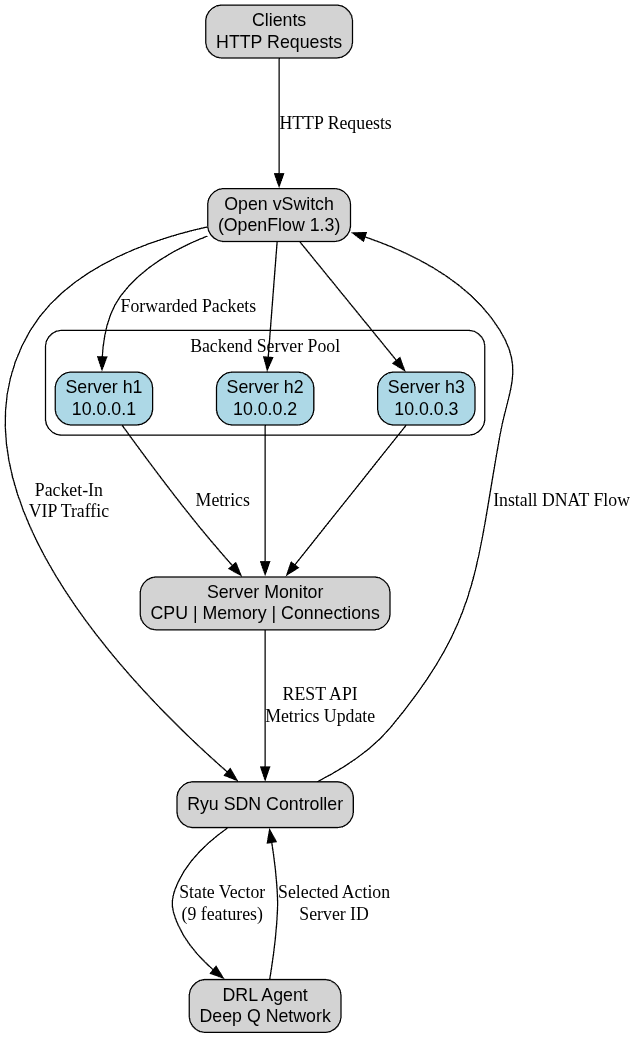
\includegraphics[width=0.25\linewidth]{Images/arch.png}
    \caption{DRL-SDN System Architecture}
\end{figure}
\end{frame}

% ================= TRAINING METRICS =================
\begin{frame}{Training Metrics}

\begin{figure}
    \centering
    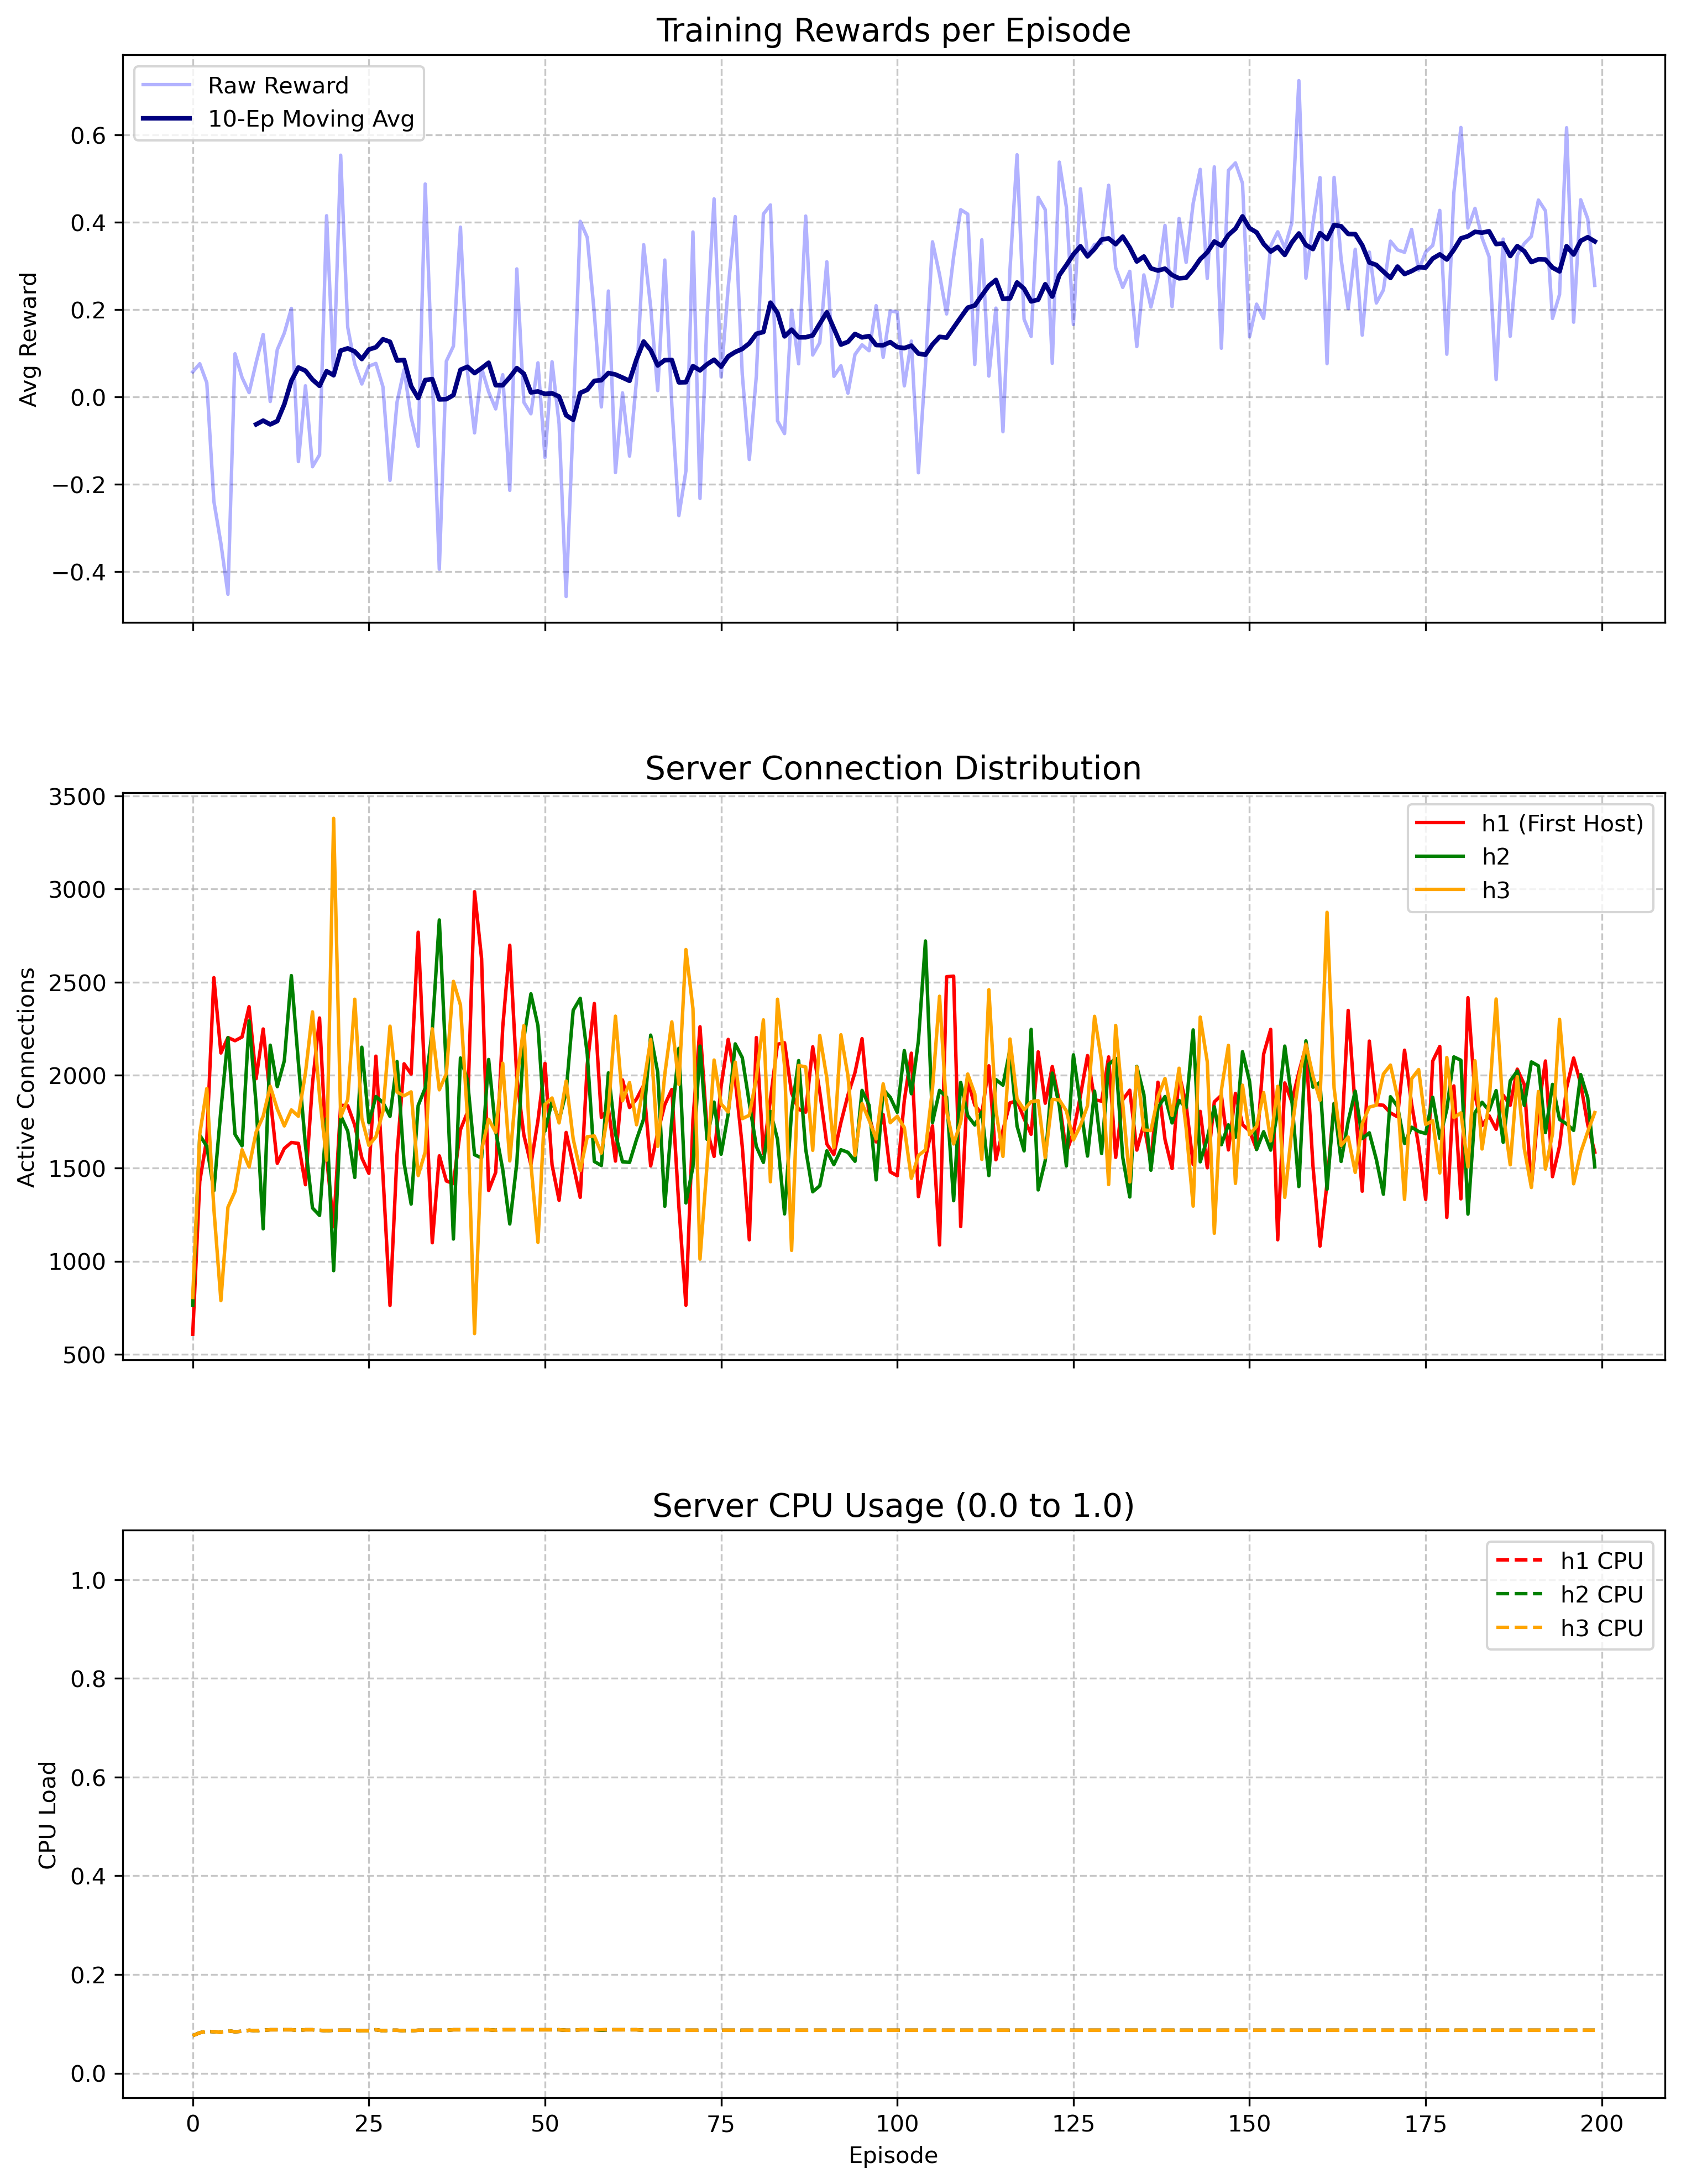
\includegraphics[width=0.55\linewidth]{Images/training_summary.png}
    \caption{Training Metrics Over Episodes}
\end{figure}
\end{frame}

% ================= CHECKPOINTING =================
\begin{frame}{Model Checkpointing}
\begin{itemize}
    \item Model saved every 10 episodes
    \item Evaluation run every 20 episodes ($\epsilon=0$)
    \item Final model stored after training
    \item Logs saved as JSON for analysis
\end{itemize}
\end{frame}

% ================= INFERENCE =================
\begin{frame}{Inference Mode (Evaluation)}
\begin{itemize}
    \item Exploration disabled ($\epsilon = 0$)
    \item Agent acts purely on learned policy
    \item Traffic: 80 requests/sec for 120 seconds
    \item System polled every second
\end{itemize}
\end{frame}

% ================= INFERENCE RESULTS =================
\begin{frame}{Inference Results}
\begin{figure}
    \centering
    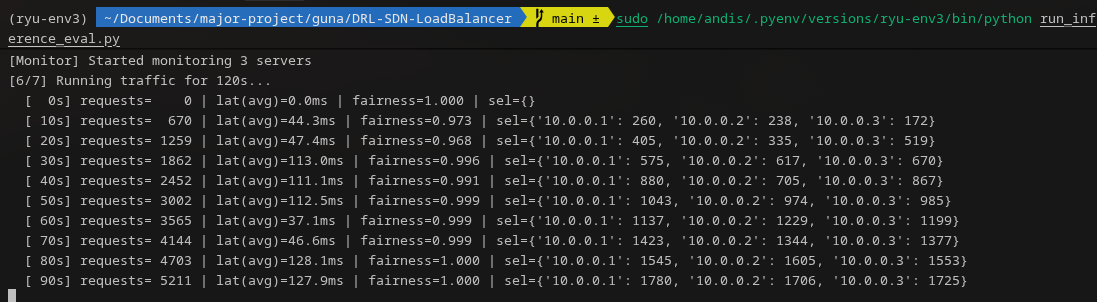
\includegraphics[width=0.85\linewidth]{Images/inference.png}
    \caption{Evaluation Output}
\end{figure}
\end{frame}

\begin{frame}{Inference Results}
\begin{figure}
    \centering
    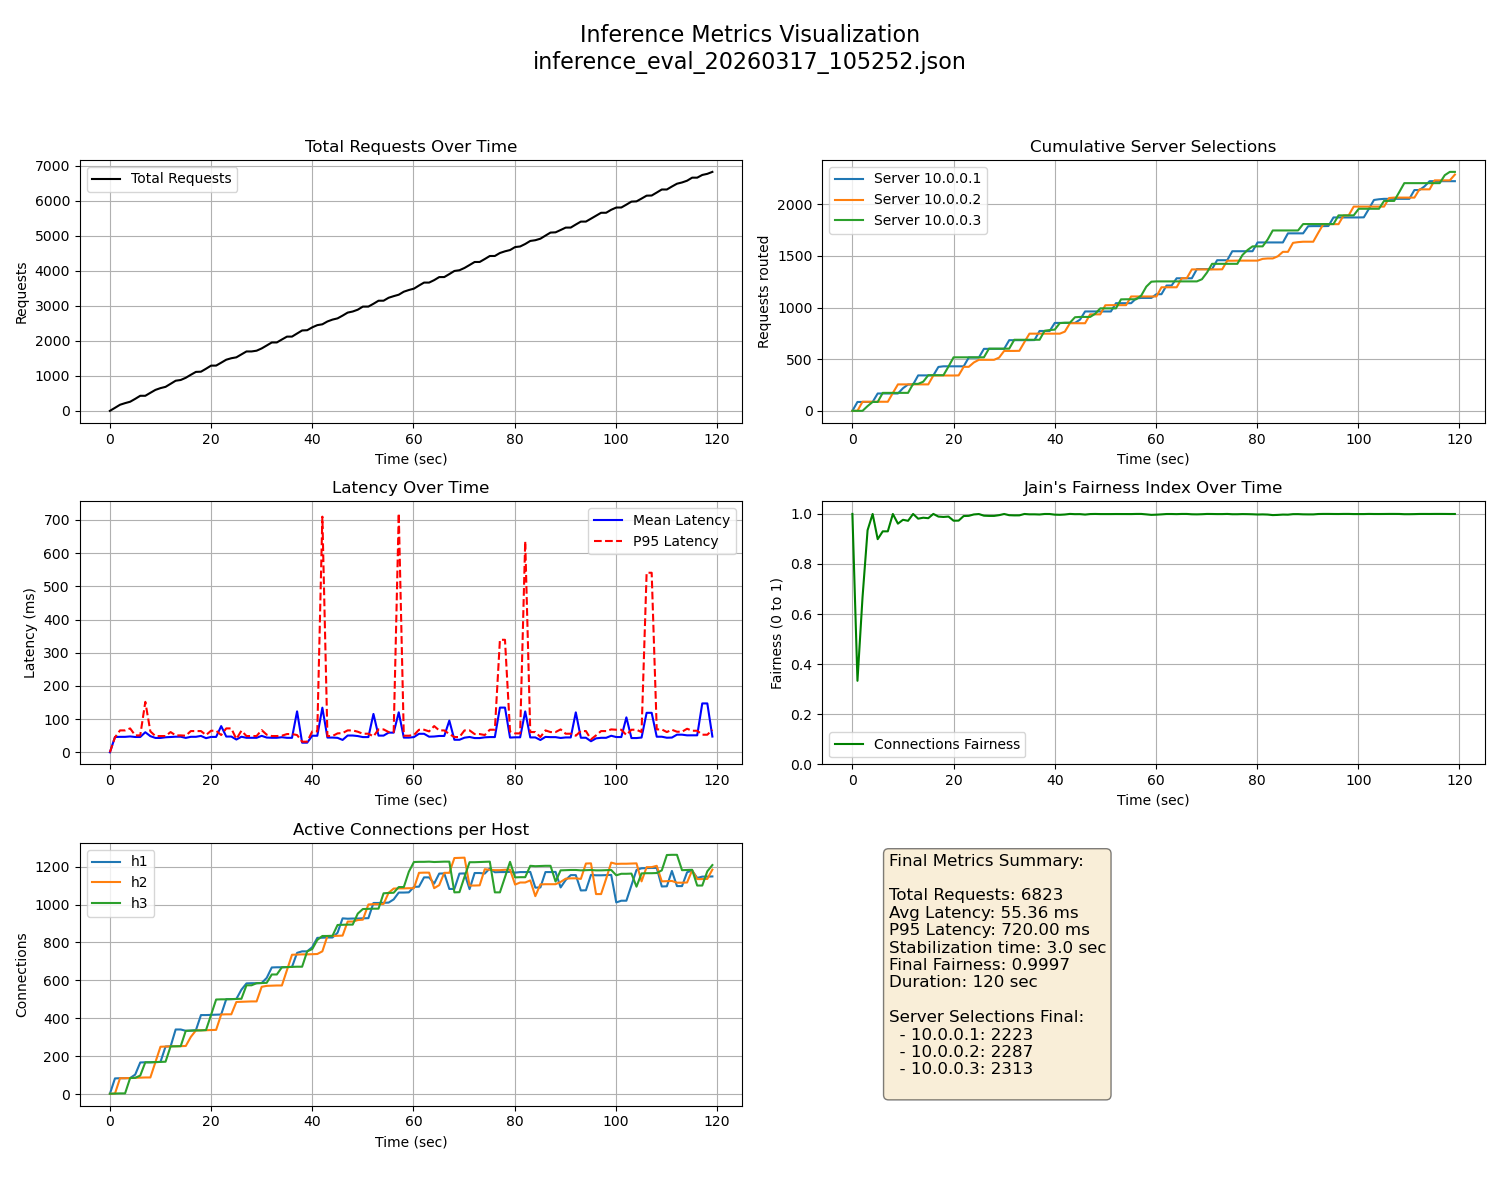
\includegraphics[width=0.85\linewidth]{Images/inference_plot.png}
    \caption{Results During Evaluation}
\end{figure}
\end{frame}



% ================= OBSERVATIONS =================
\begin{frame}{Observations}
\begin{itemize}
    \item Agent learns near-uniform load distribution
    \item Reward stabilizes across episodes
    \item Latency improves compared to naive routing
    \item System adapts to traffic variations
\end{itemize}
\end{frame}

% ================= LIMITATIONS =================
\begin{frame}{Current Limitations}
\begin{itemize}
    \item Simulation-only evaluation using Mininet
    \item Single SDN controller (Ryu)
    \item Synthetic traffic generation (Apache Bench)
    \item No deployment on real SDN hardware
    \item Small-scale topology (3 servers)
    \item Delays in metric collection
    \item Hyperparameter sensitivity
    \item Mininet lacks hardware-level realism
\end{itemize}
\end{frame}


% ================= SUMMARY =================
\begin{frame}{Summary of Accomplishments}
\begin{itemize}
    \item Complete DRL-SDN pipeline implemented
    \item MDP formulation and DQN training completed
    \item Real traffic-based training executed
    \item Inference evaluation with fairness and latency metrics
    \item System ready for benchmarking and scaling
\end{itemize}
\end{frame}
